\section{Quiz Bowl Playing Robot}

\begin{frame}
	\frametitle{System for Incremental Classifiers}

	\begin{itemize}
		\item Treat this as a MDP
		\item Action: {\bf buzz} now or {\bf wait}
                     \pause
                    \begin{enumerate}
                  \item {\bf Content Model} is constantly generating guesses
                     \item {\bf Oracle} provides examples where it is correct
                   \item The {\bf Policy} generalizes to test data
                       \item {\bf Features} represent our state
                    \end{enumerate}
	\end{itemize}
\begin{block}{}
  \begin{center}
    \vspace{-.5cm}
    \begin{tabular}{cccc}
      \alert<3->{content model} & oracle & policy & features \\
    \end{tabular}
    \vspace{-.5cm}
  \end{center}
\end{block}
\end{frame}


\begin{frame}{Content Model}

\begin{block}{}
  \begin{center}
    \vspace{-.5cm}
    \begin{tabular}{cccc}
      \alert{content model} & oracle & policy & features \\
    \end{tabular}
    \vspace{-.5cm}
  \end{center}
\end{block}


  \begin{itemize}
   \item Bayesian generative model with answers as latent state
         \item Unambiguous Wikipedia pages
           \item Na\"ive Bayes
    \item Maintains posterior distribution over guesses
    \item Always has a guess of what it should answer
      \begin{itemize}
        \item policy will tell us when to trust it
       \end{itemize}

  \end{itemize}
\end{frame}

\begin{frame}{Oracle}
\begin{block}{}
  \begin{center}
    \vspace{-.5cm}
    \begin{tabular}{cccc}
      content model & \alert{oracle} & policy & features \\
    \end{tabular}
    \vspace{-.5cm}
  \end{center}
\end{block}
\begin{center}
  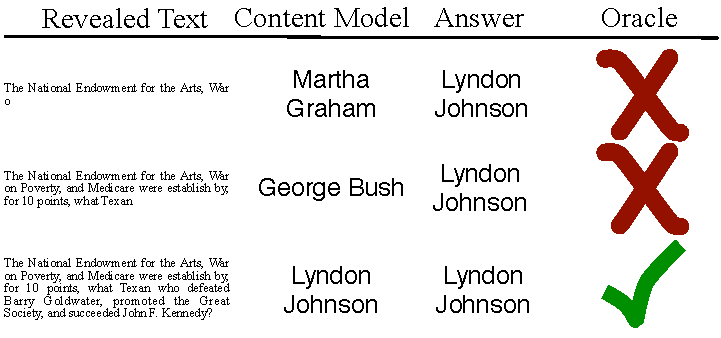
\includegraphics[width=0.8\linewidth]{qb/oracle}
\end{center}

\begin{itemize}
  \item As each token is revealed, look at content model's guess
    \item If it's right, positive instance; otherwise negative
      \item Nearly optimal policy to buzz whenever correct (upper bound)
\end{itemize}

\end{frame}

\begin{frame}{Policy}

\begin{block}{}
  \begin{center}
    \vspace{-.5cm}
    \begin{tabular}{cccc}
      content model & oracle & \alert{policy} & features \\
    \end{tabular}
    \vspace{-.5cm}
  \end{center}
\end{block}

 \begin{itemize}
    \item Mapping: state $\mapsto$ action
    \item Use oracle as example actions
    \item Learned as classifier \cite{langford-05}
    \item At test time, use the same features as for training
      \begin{itemize}
        \item Question text (so far)
        \item Guess
        \item Posterior distribution
        \item Change in posterior
      \end{itemize}
\end{itemize}

\end{frame}



\begin{frame}[t]{Features (by example)}

\only<1-3>{
\begin{block}{}
  \begin{center}
    \vspace{-.5cm}
    \begin{tabular}{cccc}
      content model & oracle & policy & \alert{features} \\
    \end{tabular}
    \vspace{-.5cm}
  \end{center}
\end{block}
\vspace{.5cm}
}

  \begin{columns}[T]
    \column{.3\linewidth}

    \only<1->{ 
\includegraphics[width=2\linewidth]{qb/feature_ex_l_1} \\ }
    \vspace{.5cm}
    \only<4->{ 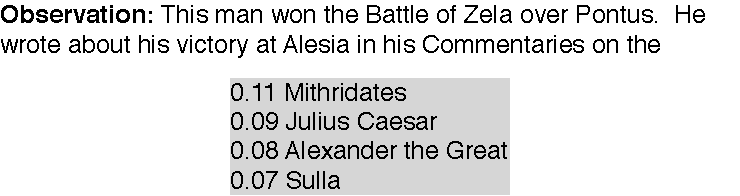
\includegraphics[width=2\linewidth]{qb/feature_ex_l_2}  \\ }
    \vspace{.5cm}
    \only<7->{ 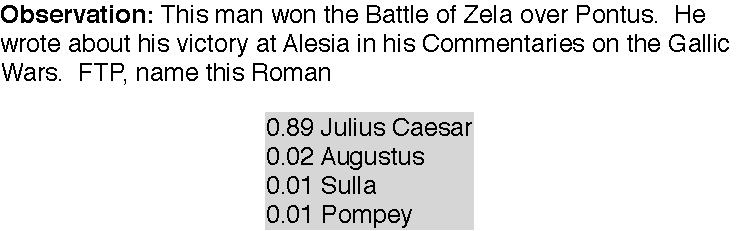
\includegraphics[width=2\linewidth]{qb/feature_ex_l_3}  \\ }


    \column{.68\linewidth}
    \vspace{-.5cm}
    \only<2->{ 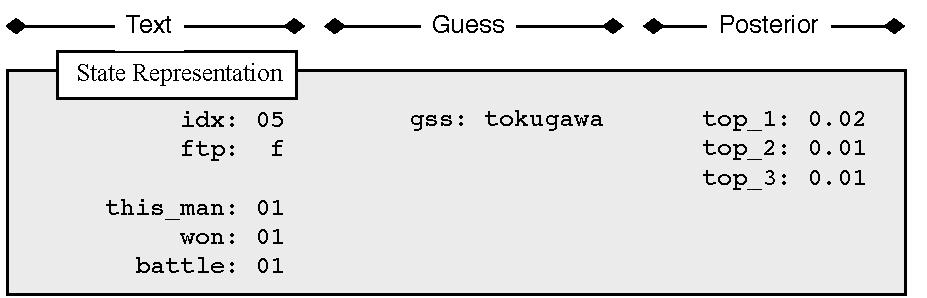
\includegraphics[width=.85\linewidth]{qb/feature_ex_r_1} \\ }
    \only<3->{ \vspace{-.5cm} \hspace{.5cm} 
\includegraphics[width=.1\linewidth]{qb/feature_ex_wait}  \\ }
    \only<5->{ 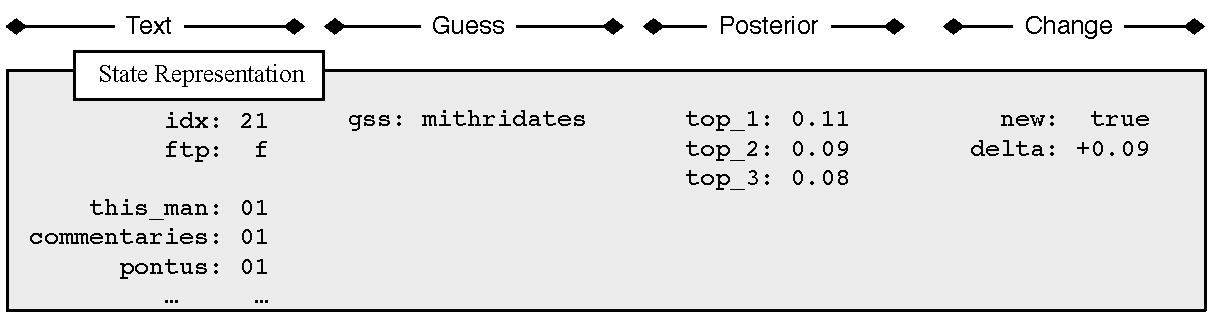
\includegraphics[width=\linewidth]{qb/feature_ex_r_2} \\ }
    \only<6->{ \vspace{-.5cm} \hspace{.5cm}
\includegraphics[width=.1\linewidth]{qb/feature_ex_wait}  \\ }
    \only<8->{ 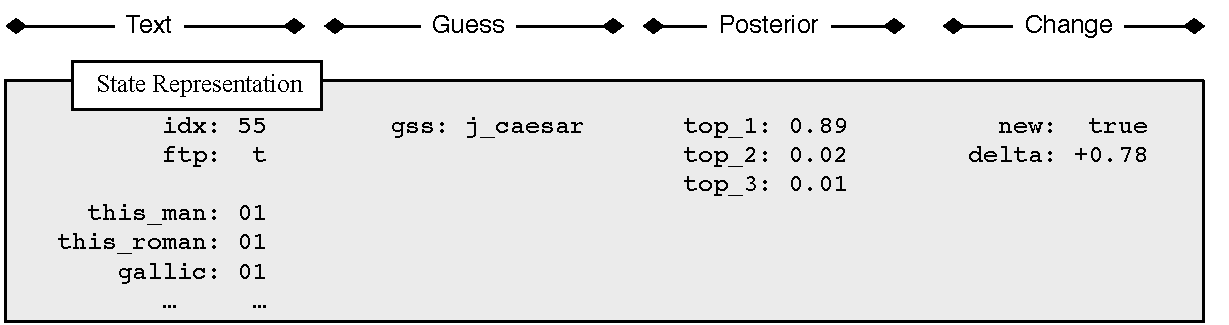
\includegraphics[width=\linewidth]{qb/feature_ex_r_3} \\ }
    \only<9->{ \vspace{-.5cm} \hspace{.5cm} 
\includegraphics[width=.1\linewidth]{qb/feature_ex_buzz}  \\ }
    \only<9->{Answer: {\bf Julius Caesar}}
  \end{columns}

\end{frame}



\begin{frame}{Simulating a Game}
		\begin{itemize}
			\item Present tokens incrementally to algorithm, see where it buzzes
			\item Compare to where humans buzzed in
			\item Payoff matrix (wrt Computer)
			\begin{center}
\begin{tabular}{lccr}
& Computer & Human & Payoff \\
\hline
1 & first and wrong & right & $-15$ \\
2 & --- & first and correct & $-10$ \\
3  & first and wrong & wrong & $-5$ \\
4 & first and correct & --- & $+10$ \\
5 & wrong & first and wrong & $+5$ \\
6 & right & first and wrong & $+15$ \\
\hline
\end{tabular}
			\end{center}
		\end{itemize}
\end{frame}

\iflong

\begin{frame}[t]
	\frametitle{Race Against the Machine}
	\begin{center}

\begin{tabular}{|ll|ccc|c|}
\hline
      &   & \multicolumn{3}{c|}{Human Scoring} & \\
Strategy&	Features & \alert<1>{Average} &	\alert<2>{Best}&	\alert<3>{Median} &	Token\\
\hline
\multirow{4}{*}{Classify}
& text & -8.72 & -10.04 & -6.50 & 40.36 \\
& +guess & -5.71 & -8.40 & -3.95 & 66.02 \\
& +pos & -4.13 & -7.56 & -2.70 & 67.97 \\
& \alert<5>{+change} & {\bf -4.02} & {\bf -7.41} & {\bf -2.63} & 77.33 \\
\hline
\alert<6>{Oracle} &  & 3.36 & 0.61 & 4.35 & 49.90 \\
\hline
                      & \alert<7>{all}             & -6.61         & -9.03         & -4.42 & 100.19 \\
                     & \alert<8>{ftp}              & -5.22         & -8.62         & -4.23 & 88.65 \\
Rapacious             &  \alert<9>{index$_{30}$}   & -7.89         & -8.71         & -6.41 & 32.23 \\
Baseline         &  \alert<9>{index$_{60}$ }       & -5.16         & {\bf -7.56}   & -3.71 & 61.90 \\
                      & \alert<9>{ index$_{90}$ }  & {\bf -5.02}   & -8.62         & {\bf -3.50} & 87.13 \\
\hline
\end{tabular}
	\end{center}
\vspace{-1cm}
% \only<4>{ \paragraph{token} Where the algorithm buzzed in.}
\only<6>{ \paragraph{Oracle} Best possible incremental strategy \emph{post hoc}}
\only<5>{ \paragraph{Classify} Incremental algorithms doing best, but not that well}
\only<7>{ \paragraph{all} This strategy waits until the end of the question and answers the best
  answer possible.}
\only<8>{ \paragraph{ftp} Waiting until when ``for 10 points'' is said, then giving the
    best answer possible.}
\only<9>{ \paragraph{index-n} Waiting until the first feature after the $n^{th}$ token has been processed, then giving the best answer possible.  }
\only<1> { \paragraph{average} For each human who answered a question, compare the positions and compute a reward.  Average them.}
\only<2> { \paragraph{best} For each question, take the human buzz position to be the the
  earliest that \emph{any} human buzzed in the question}
\only<3> { \paragraph{median} For each question, take the human buzz position to be the
  earliest position after 50\% of human buzzes appeared.}
\end{frame}


\else

\begin{frame}{Simulating a Game}

  \begin{itemize}
    \item What human actions to compare against?
      \invisible<1>{
      \begin{itemize}
        \item On each question, take the {\bf median} buzz (more in paper)
      \end{itemize}
      }
     \item Does it to better than obvious rapacious baselines?
      \invisible<-2>{
        \begin{itemize}
          \item Yes---experiments in paper
          \end{itemize}
        }
    \item How do features affect performance?
      \invisible<-3>{
      \begin{itemize}
        \item Nothing hurts, but only a handful help (details in paper)
      \end{itemize}
      }
  \end{itemize}

  \invisible<-4>{.}

\end{frame}


\begin{frame}{How does a na\"ive content model do?}
\begin{center}
\begin{tabular}{ll|c|c}
Strategy &  Model    &	Points &	Index\\
\hline
\multirow{4}{*}{Classify}
& na\"ive & -1.63 & 77.33 \\
& & & \\
& & & \\
& & & \\
\hline
\end{tabular}
\end{center}

\end{frame}

\fi

